\documentclass{article}
\usepackage{geometry}
\usepackage{graphicx}
\renewcommand{\familydefault}{\sfdefault}
\usepackage{helvet}
\title{Assignment 2}
\author{Joe Brew}
\usepackage{Sweave}
\begin{document}
\newgeometry{margin=1.5cm}
\Sconcordance{concordance:ass2.tex:ass2.Rnw:%
1 7 1 1 0 5 1 1 6 18 1 1 4 1 2 4 1 1 4 1 2 2 1}

\maketitle



\section*{Note to Professor}
Dr. Cantrell,
\\ 
As with the first assignment, I completed assignment 2 entirely in R.  This is because I was not able to get SAS until Tuesday (the day before deadline).  Thank you for your understanding.

\vspace{50mm}

\tableofcontents
\newgeometry{margin=1.5cm}

\begin{center}
\section*{Side-by-side boxplots}
\end{center}
\addcontentsline{toc}{section}{Side-by-side boxplots}

\subsection*{SYSBP by SEX}
\addcontentsline{toc}{subsection}{SYSBP by SEX}
\begin{center}
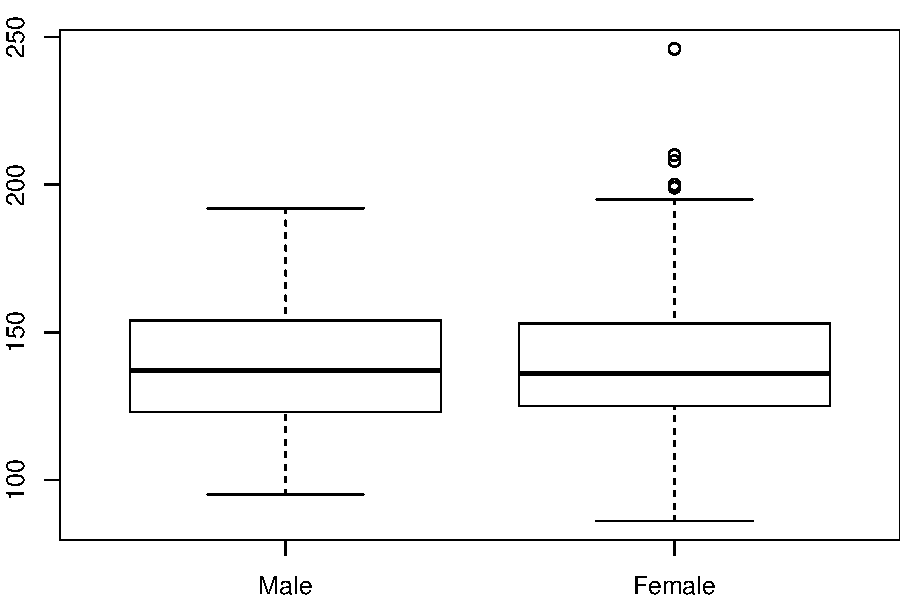
\includegraphics{ass2-002}
\end{center}

\subsection*{SYSBP by BMI}
\addcontentsline{toc}{subsection}{SYSBP by BMI}
\begin{center}
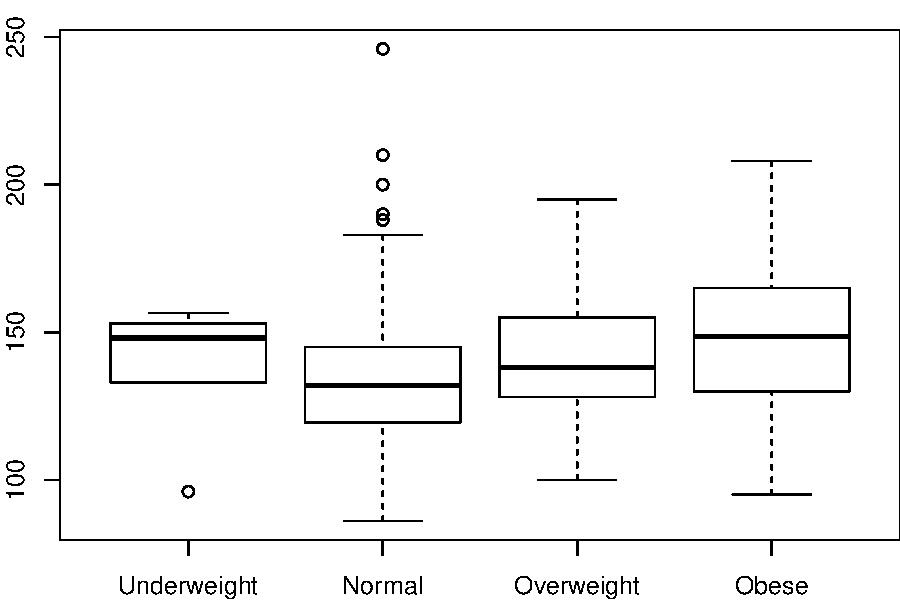
\includegraphics{ass2-003}
\end{center}
\end{document}

